\documentclass[11pt,a4paper]{article}

% --- Core Typography & Encoding ---
\usepackage[utf8]{inputenc}
\usepackage[T1]{fontenc}
\usepackage{lmodern}
\usepackage{microtype}

% --- Mathematics & Units ---
\usepackage{amsmath,amssymb}

% --- Geometry & Page Setup ---
\usepackage[a4paper,top=2.5cm,bottom=2.5cm,left=2.3cm,right=2.3cm,headheight=14pt]{geometry}

% --- Figures & Tables ---
\usepackage{graphicx}
\usepackage{booktabs}
\usepackage{caption}
\usepackage{subcaption}
\usepackage{float}

% --- Colors & Styling ---
\usepackage{xcolor}
\definecolor{primary}{RGB}{0, 43, 91}       % Navy Blue
\definecolor{secondary}{RGB}{0, 102, 178}   % Academic Blue
\definecolor{darkgray}{RGB}{50, 50, 50}
\definecolor{lightgray}{RGB}{245, 247, 250}
\definecolor{bordercolor}{RGB}{210, 220, 230}

% --- Callout Boxes & Headings ---
\usepackage[most]{tcolorbox}
\usepackage{titlesec}
\usepackage{fancyhdr}
\usepackage{hyperref}

% --- Heading Formatting ---
\titleformat{\section}
  {\color{primary}\Large\bfseries}{\thesection}{1em}{}[\titlerule]
\titleformat{\subsection}
  {\color{secondary}\large\bfseries}{\thesubsection}{1em}{}
\titleformat{\subsubsection}
  {\color{darkgray}\normalsize\bfseries}{\thesubsubsection}{1em}{}

% --- Header & Footer ---
\pagestyle{fancy}
\fancyhf{}
\fancyhead[L]{\small\color{darkgray}\textit{NACA 23015 Airfoil Aerodynamic CFD Analysis}}
\fancyhead[R]{\small\color{darkgray}\textit{Fluid Mechanics II}}
\fancyfoot[C]{\thepage}
\renewcommand{\headrulewidth}{0.4pt}
\renewcommand{\footrulewidth}{0pt}

% --- Hyperlink Settings ---
\hypersetup{
    colorlinks=true,
    linkcolor=secondary,
    citecolor=secondary,
    urlcolor=secondary,
    pdftitle={Aerodynamic Analysis and Validation of the NACA 23015 Airfoil},
    pdfauthor={Ali Taheri (ID: 401170875)},
    pdfsubject={Fluid Mechanics II Project Report}
}

% --- Custom Info Box ---
\newtcolorbox{academicbox}[1][]{
  colback=lightgray,
  colframe=secondary,
  arc=3mm,
  boxrule=1pt,
  fonttitle=\bfseries\color{white},
  coltitle=white,
  colbacktitle=secondary,
  enhanced,
  attach boxed title to top left={yshift=-2mm,xshift=5mm},
  title=#1
}

\begin{document}

% ==============================================================================
% COVER PAGE
% ==============================================================================
\begin{titlepage}
    \hypersetup{pageanchor=false}
    \centering
    \vspace*{0.5cm}
    
    % Institutional / Department Header
    {\large Department of Mechanical Engineering \par}
    \vspace{0.4cm}
    {\color{secondary}\rule{\textwidth}{1.5pt}}
    \vspace{1.5cm}
    
    % Main Document Title
    {\Huge\bfseries\color{primary} Aerodynamic Analysis and Validation of the NACA 23015 Airfoil \par}
    \vspace{0.6cm}
    
    % Subtitle
    {\Large\color{darkgray} A Numerical CFD Study on Grid Independence, Flow Physics, and Turbulence Modeling in ANSYS Fluent \par}
    
    \vspace{1.8cm}
    
    % Representative Domain Graphic
    \begin{center}
        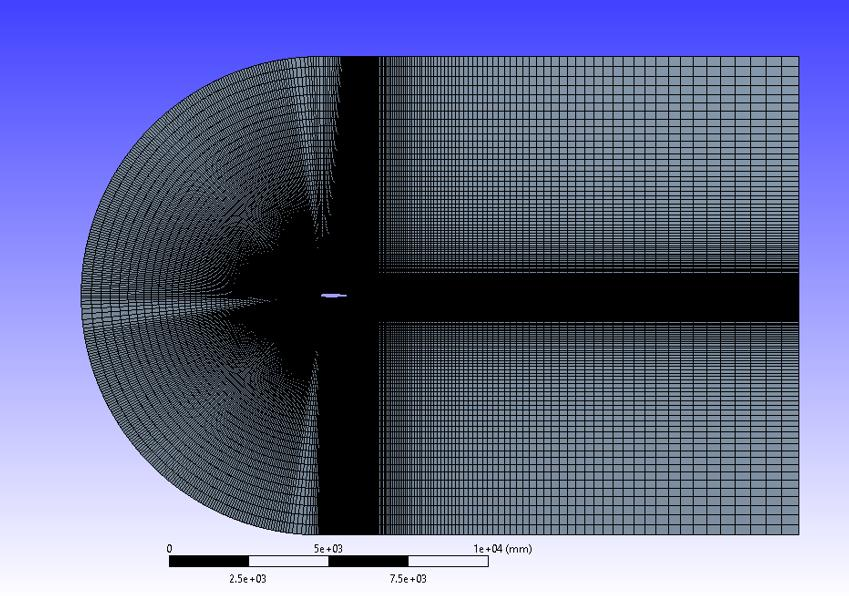
\includegraphics[width=0.68\textwidth]{report_figures/domain_mesh.png}\\[0.5em]
        {\small\color{darkgray}\textit{Computational C-grid mesh domain around the NACA 23015 profile}}
    \end{center}
    
    \vfill
    
    % Author & Project Metadata Block
    \begin{tcolorbox}[colback=lightgray,colframe=bordercolor,arc=2mm,boxrule=1pt,width=0.9\textwidth]
        \centering
        \vspace{0.2cm}
        \begin{tabular}{rl}
            \textbf{Author:} & \textbf{Ali Taheri} \\[0.3em]
            \textbf{Student ID:} & \textbf{401170875} \\[0.3em]
            \textbf{Course:} & Fluid Mechanics II \\[0.3em]
            \textbf{Simulation Software:} & ANSYS Workbench 2019 R1 / ANSYS Fluent \\[0.3em]
            \textbf{Date:} & September 2026 / Academic Term 2025--2026 \\
        \end{tabular}
        \vspace{0.2cm}
    \end{tcolorbox}
    
    \vspace{0.8cm}
\end{titlepage}

% ==============================================================================
% EXECUTIVE SUMMARY & TABLE OF CONTENTS
% ==============================================================================
\hypersetup{pageanchor=true}
\pagenumbering{roman}

\begin{abstract}
\noindent This report presents a comprehensive numerical simulation and aerodynamic analysis of external incompressible flow past a 2D \textbf{NACA 23015} airfoil. The simulation was performed in \textbf{ANSYS Fluent 2019 R1} using a structured C-grid computational topology. A systematic grid convergence study was conducted across three spatial resolutions (coarse: 7,800 elements; medium: 81,300 elements; fine: 199,500 elements), demonstrating that the medium mesh achieves asymptotic grid independence with a lift coefficient deviation of only $1.3\%$ relative to the fine grid. Aerodynamic lift and drag coefficients at an angle of attack $\alpha = 6^\circ$ were validated against empirical wind tunnel polar data from Abbott \& von Doenhoff ($C_l = 0.612$ vs. $\approx 0.70$). Comparative analyses were conducted between laminar and turbulent ($k\text{-}\omega\text{ SST}$) regimes at $\alpha = 10^\circ$, demonstrating that absent turbulent momentum diffusion, laminar flow experiences premature boundary layer separation, resulting in stall and severe drag escalation. Furthermore, detailed flow field contours (static pressure, dynamic pressure, velocity magnitude, vorticity, streamlines, and surface pressure coefficients $C_p$) are evaluated at $\alpha = 6^\circ$ and $\alpha = 10^\circ$, elucidating boundary layer growth, adverse pressure gradient effects, and incipient separation mechanisms.
\end{abstract}

\vspace{0.8cm}
\tableofcontents
\newpage

\pagenumbering{arabic}

% ==============================================================================
% SECTION 1: INTRODUCTION & AIRFOIL GEOMETRY
% ==============================================================================
\section{Introduction and Geometric Modeling}
The \textbf{NACA 23015} is a 5-digit cambered airfoil renowned in aeronautical engineering for generating high maximum lift coefficients with exceptionally low pitching moments ($C_{m,c/4}$), making it a favored design for transport wings and general aviation aircraft. The 5-digit designation indicates:
\begin{itemize}
    \item \textbf{2}: Design lift coefficient $C_{l,\text{design}} = 0.3$ ($2 \times 0.15$).
    \item \textbf{30}: Position of maximum camber along the chord ($x/c = 0.15$, forward camber location).
    \item \textbf{15}: Maximum thickness-to-chord ratio of $15\%$ ($t/c = 0.15$).
\end{itemize}

The airfoil profile coordinates were discretized with a standard chord length $c = 1000\text{ mm} = 1.0\text{ m}$ and exported in both comma-separated (\texttt{NACA23015.csv}) and tab-delimited formats (\texttt{NACA23015.txt}) compatible with ANSYS DesignModeler 3D curve generation.

% ==============================================================================
% SECTION 2: COMPUTATIONAL DOMAIN & BOUNDARY CONDITIONS
% ==============================================================================
\section{Computational Domain and Boundary Conditions}
To eliminate artificial boundary reflection and ensure authentic freestream flow development, a classical \textbf{C-grid} domain was constructed surrounding the airfoil:
\begin{itemize}
    \item \textbf{Inlet Boundary (C-arc):} Semi-circular arc placed $10c$ upstream from the airfoil leading edge, prescribed as a \textit{Velocity Inlet} with uniform velocity, standard atmospheric air density ($\rho = 1.225\text{ kg/m}^3$), and dynamic viscosity ($\mu = 1.802 \times 10^{-5}\text{ kg/(m}\cdot\text{s)}$).
    \item \textbf{Outlet Boundary:} Rectangular wake domain extending $15c$ downstream of the trailing edge, prescribed as a \textit{Pressure Outlet} ($p_{\text{gauge}} = 0\text{ Pa}$).
    \item \textbf{Airfoil Surface:} Prescribed as a stationary, no-slip boundary wall ($u = v = 0$).
    \item \textbf{Upper and Lower Farfield:} Bounding walls set with zero-gradient or freestream slip conditions.
\end{itemize}

\begin{figure}[H]
    \centering
    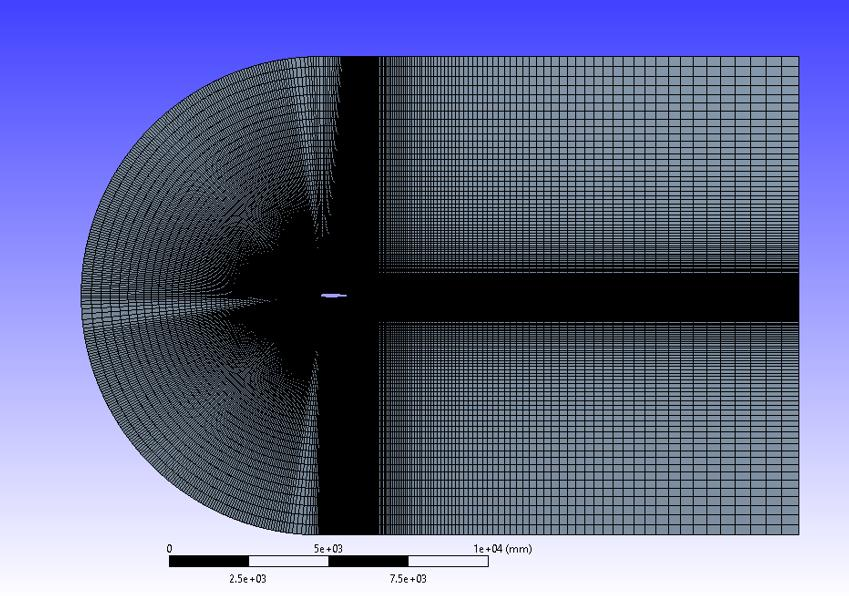
\includegraphics[width=0.85\textwidth]{report_figures/domain_mesh.png}
    \caption{Computational C-grid mesh domain around the NACA 23015 profile in ANSYS Meshing.}
    \label{fig:domain_mesh}
\end{figure}

The baseline solver utilizes the two-equation \textbf{$k\text{-}\omega\text{ SST}$ (Shear Stress Transport)} turbulence model, combining the robust near-wall accuracy of the Wilcox $k\text{-}\omega$ formulation with the freestream independence of the $k\text{-}\epsilon$ model. Double-precision arithmetic was applied with second-order upwind spatial discretization for momentum, turbulent kinetic energy, and specific dissipation rate.

% ==============================================================================
% SECTION 3: MESH INDEPENDENCE STUDY
% ==============================================================================
\section{Mesh Independence Study}
To ensure that numerical solutions are free from spatial discretization errors, three grids of varying densities were constructed and evaluated under identical boundary conditions at an angle of attack $\alpha = 6^\circ$:
\begin{enumerate}
    \item \textbf{Coarse Mesh:} 7,800 elements, 7,956 nodes.
    \item \textbf{Medium Mesh:} 81,300 elements, 81,892 nodes.
    \item \textbf{Fine Mesh:} 199,500 elements, 200,398 nodes.
\end{enumerate}

Convergence histories for lift coefficient ($C_l$) and drag coefficient ($C_d$) are illustrated in Figures~\ref{fig:mid_convergence} and \ref{fig:fine_convergence}, while residual convergence for the coarse mesh is depicted in Figure~\ref{fig:coarse_residuals}.

\begin{figure}[H]
    \centering
    \begin{subfigure}[b]{0.48\textwidth}
        \centering
        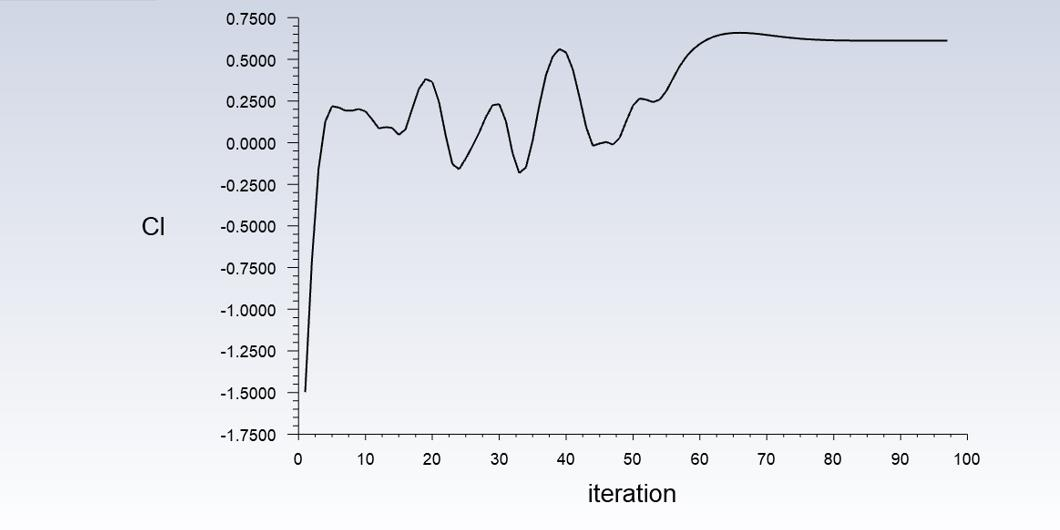
\includegraphics[width=\textwidth]{report_figures/cl_mid_mesh.png}
        \caption{$C_l$ vs. Iterations (Medium Mesh)}
    \end{subfigure}
    \hfill
    \begin{subfigure}[b]{0.48\textwidth}
        \centering
        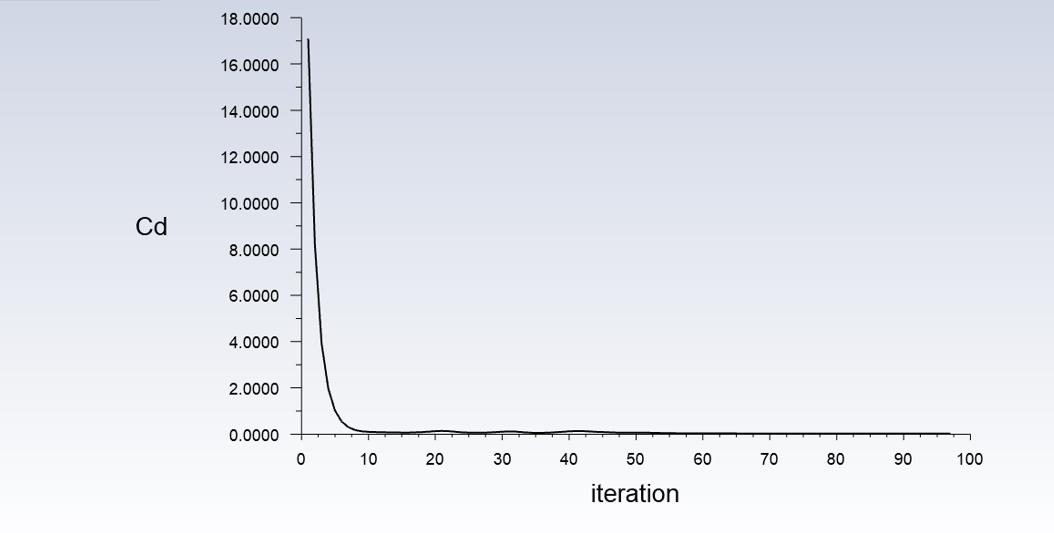
\includegraphics[width=\textwidth]{report_figures/cd_mid_mesh.png}
        \caption{$C_d$ vs. Iterations (Medium Mesh)}
    \end{subfigure}
    \caption{Iterative convergence monitors for the Medium Mesh ($81,300$ elements): $C_l = 0.612$, $C_d = 0.028$.}
    \label{fig:mid_convergence}
\end{figure}

\begin{figure}[H]
    \centering
    \begin{subfigure}[b]{0.48\textwidth}
        \centering
        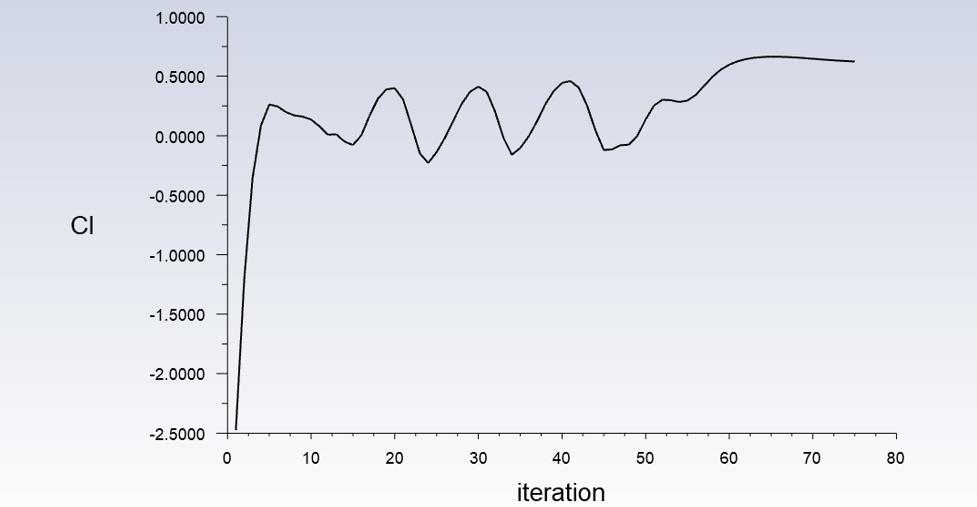
\includegraphics[width=\textwidth]{report_figures/cl_fine_mesh.png}
        \caption{$C_l$ vs. Iterations (Fine Mesh)}
    \end{subfigure}
    \hfill
    \begin{subfigure}[b]{0.48\textwidth}
        \centering
        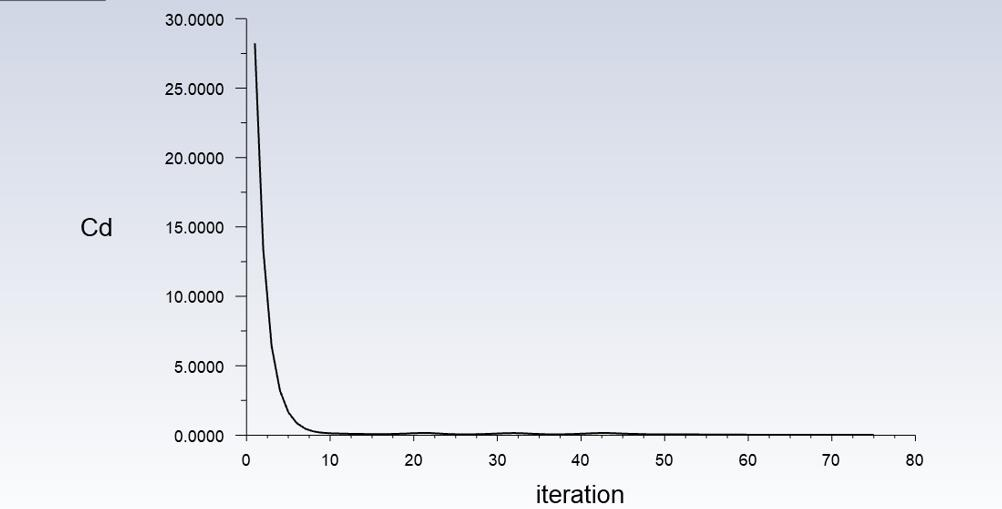
\includegraphics[width=\textwidth]{report_figures/cd_fine_mesh.png}
        \caption{$C_d$ vs. Iterations (Fine Mesh)}
    \end{subfigure}
    \caption{Iterative convergence monitors for the Fine Mesh ($199,500$ elements): $C_l = 0.620$, $C_d = 0.029$.}
    \label{fig:fine_convergence}
\end{figure}

\begin{figure}[H]
    \centering
    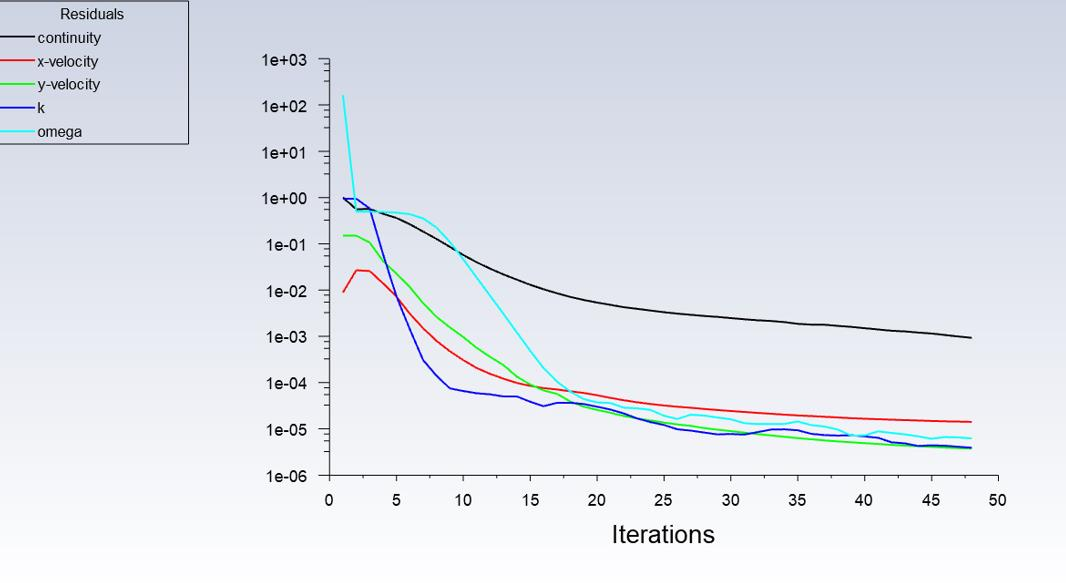
\includegraphics[width=0.72\textwidth]{report_figures/residuals_coarse_mesh.png}
    \caption{Residual convergence history (Continuity, X/Y Momentum, $k$, $\omega$) for the Coarse Mesh.}
    \label{fig:coarse_residuals}
\end{figure}

\begin{table}[H]
    \centering
    \small
    \caption{Grid Convergence Summary at Angle of Attack $\alpha = 6^\circ$.}
    \label{tab:mesh_study}
    \vspace{0.2cm}
    \begin{tabular}{lccccc}
        \toprule
        \textbf{Mesh Level} & \textbf{Elements} & \textbf{Nodes} & \textbf{Lift Coeff. ($C_l$)} & \textbf{Drag Coeff. ($C_d$)} & \textbf{Relative Error $\Delta C_l$} \\
        \midrule
        Coarse & 7,800 & 7,956 & 0.342 & 0.026 & $-44.8\%$ \\
        Medium & 81,300 & 81,892 & 0.612 & 0.028 & $-1.3\%$ \\
        Fine & 199,500 & 200,398 & 0.620 & 0.029 & \textit{Baseline} \\
        \bottomrule
    \end{tabular}
\end{table}

\begin{academicbox}[Mesh Convergence Analysis]
The analysis of the three mesh topologies demonstrates that the coarse grid produces a substantial error ($\approx 44.8\%$ underprediction in $C_l$), establishing that it lacks adequate spatial and boundary layer resolution to resolve the leading-edge suction peak. 

Conversely, refining the grid by $2.45\times$ from the medium mesh ($81.3\text{k}$) to the fine mesh ($199.5\text{k}$) results in only a marginal $1.3\%$ shift in $C_l$ and $3.5\%$ shift in $C_d$, while incurring more than double the memory consumption and solution runtime. Consequently, the \textbf{medium mesh} achieves asymptotic grid independence and is selected as the optimal computational compromise for all subsequent analyses.
\end{academicbox}

% ==============================================================================
% SECTION 4: VALIDATION AGAINST EXPERIMENTAL DATA
% ==============================================================================
\section{Verification and Validation against Experimental Data}
To validate the reliability of the CFD model, the converged simulation results at $\alpha = 6^\circ$ were compared against standard empirical wind tunnel polar data for the NACA 23015 airfoil published in Abbott \& von Doenhoff (\textit{Theory of Wing Sections}), shown in Figure~\ref{fig:validation_polar}.

\begin{figure}[H]
    \centering
    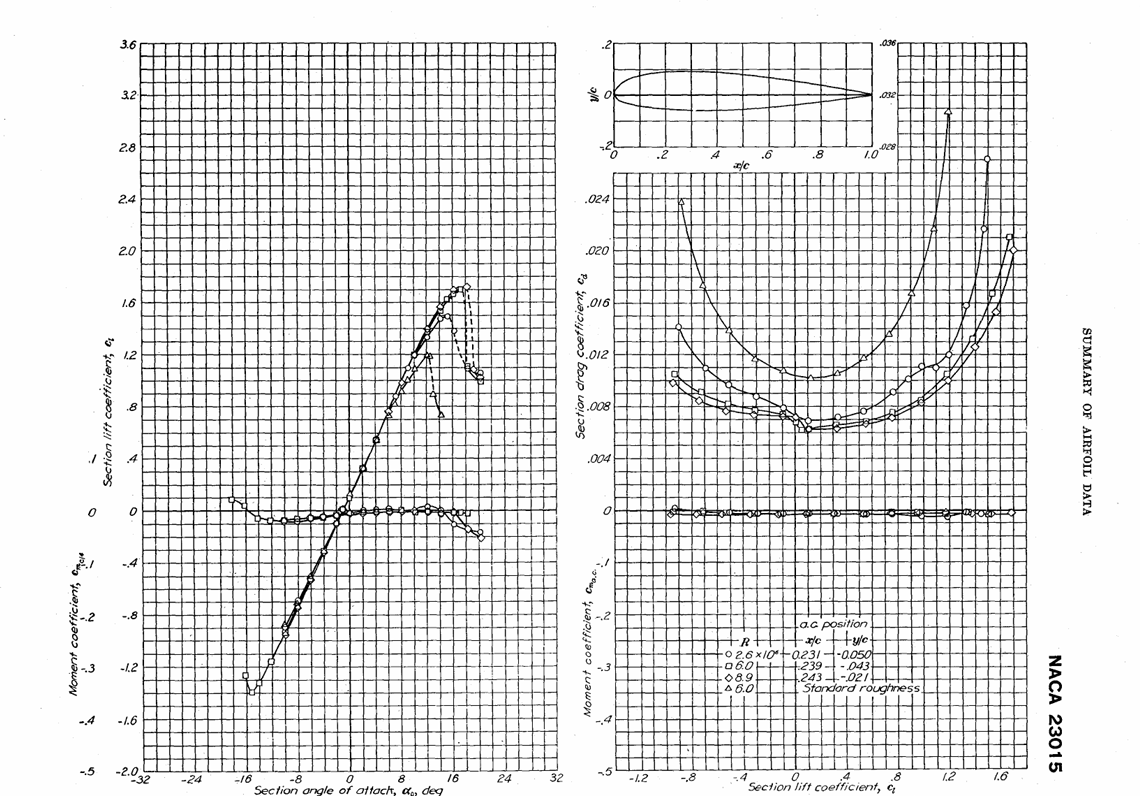
\includegraphics[width=0.65\textwidth]{report_figures/naca23015_validation_polar.png}
    \caption{Experimental aerodynamic polar chart for the NACA 23015 airfoil (Abbott \& von Doenhoff).}
    \label{fig:validation_polar}
\end{figure}

\begin{table}[H]
    \centering
    \small
    \caption{Comparison of Simulated and Experimental Aerodynamic Coefficients at $\alpha = 6^\circ$.}
    \label{tab:validation}
    \vspace{0.2cm}
    \begin{tabular}{lccc}
        \toprule
        \textbf{Aerodynamic Parameter} & \textbf{CFD Simulation} & \textbf{Experimental Reference} & \textbf{Discrepancy / Error (\%)} \\
        \midrule
        Section Lift Coefficient ($C_l$) & 0.612 & $\approx 0.700$ & $12.5\%$ \\
        Section Drag Coefficient ($C_d$) & 0.028 & $\approx 0.014$ & $\approx 50\%$ \\
        \bottomrule
    \end{tabular}
\end{table}

\begin{academicbox}[Physical Discussion on Model Discrepancies]
As observed in Table~\ref{tab:validation}, the lift coefficient exhibits acceptable agreement with experimental wind tunnel data (within $12.5\%$), but the drag coefficient is overpredicted by approximately $50\%$.

This overprediction is physically explained by the fully turbulent assumption inherent to the standard two-equation $k\text{-}\omega\text{ SST}$ model. In reality, wind tunnel tests at moderate Reynolds numbers exhibit natural laminar-to-turbulent boundary layer transition downstream of the leading edge. Assuming full turbulence right from the stagnation point induces excessive turbulent skin friction along the forward chord. Furthermore, the absence of transition models (e.g., $\gamma\text{-}Re_\theta$) and minor deviations in near-wall mesh resolution ($y^+$) account for this divergence.
\end{academicbox}

% ==============================================================================
% SECTION 5: LAMINAR VS. TURBULENT REGIMES AT AOA 10 DEG
% ==============================================================================
\section{Flow Regime Analysis: Laminar vs. Turbulent at \texorpdfstring{$\alpha = 10^\circ$}{alpha = 10 deg}}
The impact of flow turbulence on aerodynamic stability was evaluated at an angle of attack $\alpha = 10^\circ$ by simulating both pure laminar flow and fully turbulent flow ($k\text{-}\omega\text{ SST}$), as illustrated in Figure~\ref{fig:laminar_vs_turbulent}.

\begin{figure}[H]
    \centering
    \begin{subfigure}[b]{0.48\textwidth}
        \centering
        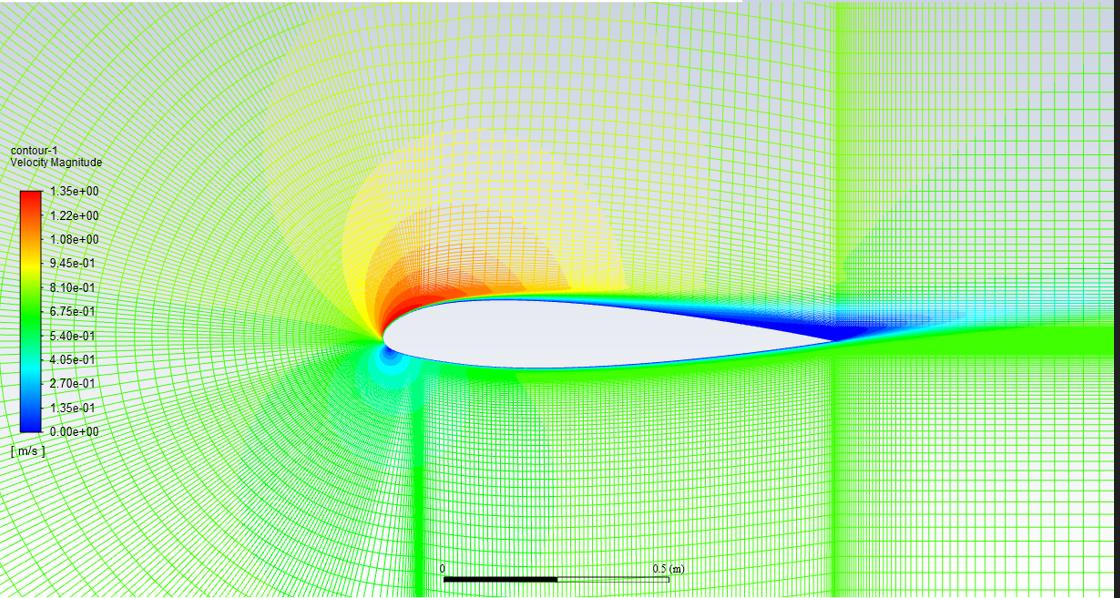
\includegraphics[width=\textwidth]{report_figures/laminar_aoa10_velocity.png}
        \caption{Laminar Regime ($\alpha = 10^\circ$)}
    \end{subfigure}
    \hfill
    \begin{subfigure}[b]{0.48\textwidth}
        \centering
        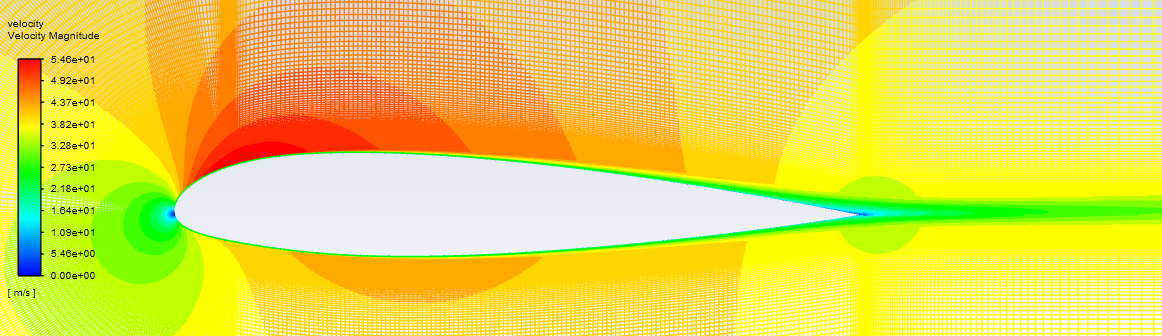
\includegraphics[width=\textwidth]{report_figures/turbulent_aoa10_velocity.png}
        \caption{Turbulent Regime ($k\text{-}\omega\text{ SST}$, $\alpha = 10^\circ$)}
    \end{subfigure}
    \caption{Comparison of velocity magnitude contours between laminar and turbulent flow regimes at $\alpha = 10^\circ$.}
    \label{fig:laminar_vs_turbulent}
\end{figure}

\paragraph{Physical Interpretation:}
In the absence of turbulence (pure laminar flow), the fluid within the boundary layer possesses significantly lower momentum. As the flow negotiates the adverse pressure gradient ($dp/dx > 0$) along the upper suction surface, the laminar boundary layer quickly runs out of kinetic energy and detaches prematurely near the forward/mid-chord region. This early separation induces massive aerodynamic stall, a catastrophic collapse in lift, and a dramatic surge in pressure (form) drag.

Conversely, in the turbulent regime, turbulent shear stresses and turbulent kinetic energy ($k$) facilitate cross-stream momentum transport from the high-speed freestream into the near-wall region. This energizes the boundary layer, allowing it to overcome the adverse pressure gradient and remain attached over a much greater chordwise fraction, preserving aerodynamic performance.

% ==============================================================================
% SECTION 6: AERODYNAMIC ANALYSIS ACROSS ANGLES OF ATTACK
% ==============================================================================
\section{Aerodynamic Flow Physics Across Angles of Attack}
As the angle of attack is increased from $\alpha = 6^\circ$ to $\alpha = 10^\circ$, the projected frontal area and vertical momentum deflection increase, resulting in a substantial augmentation of section lift. Concurrently, the adverse pressure gradient on the upper suction surface intensifies, promoting boundary layer thickening and profile drag. Although $\alpha = 10^\circ$ remains within the quasi-linear pre-stall regime for the NACA 23015 airfoil, proximity to the stall boundary reduces flow stability and increases unsteadiness.

\subsection{Static Pressure Distribution}
Figure~\ref{fig:static_pressure} compares the static pressure fields at $\alpha = 6^\circ$ and $\alpha = 10^\circ$.

\begin{figure}[H]
    \centering
    \begin{subfigure}[b]{0.48\textwidth}
        \centering
        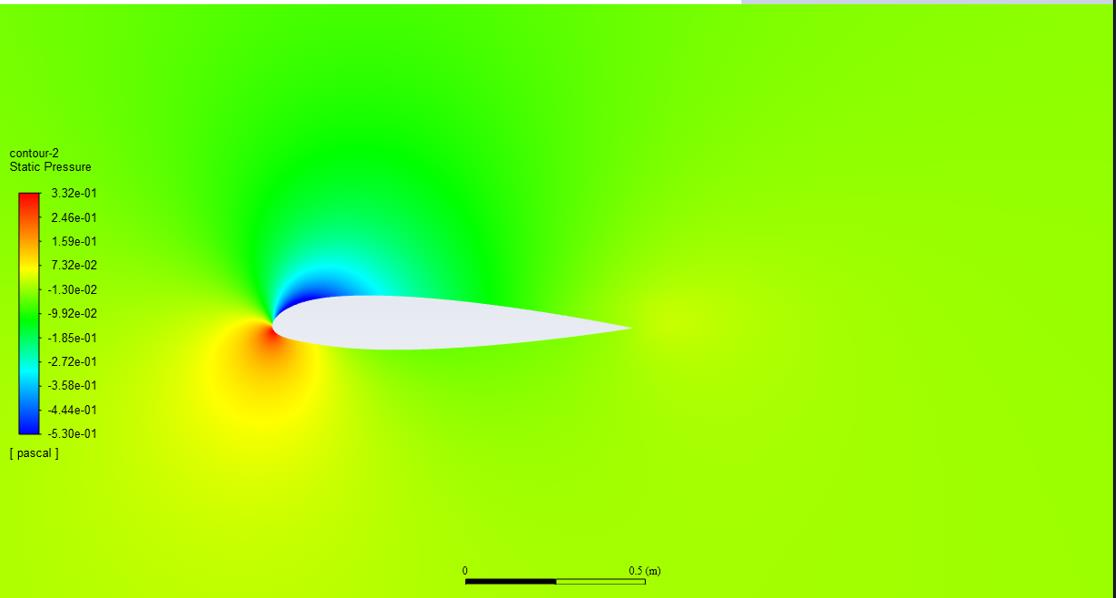
\includegraphics[width=\textwidth]{report_figures/static_pressure_aoa6.png}
        \caption{Static Pressure Contour at $\alpha = 6^\circ$}
    \end{subfigure}
    \hfill
    \begin{subfigure}[b]{0.48\textwidth}
        \centering
        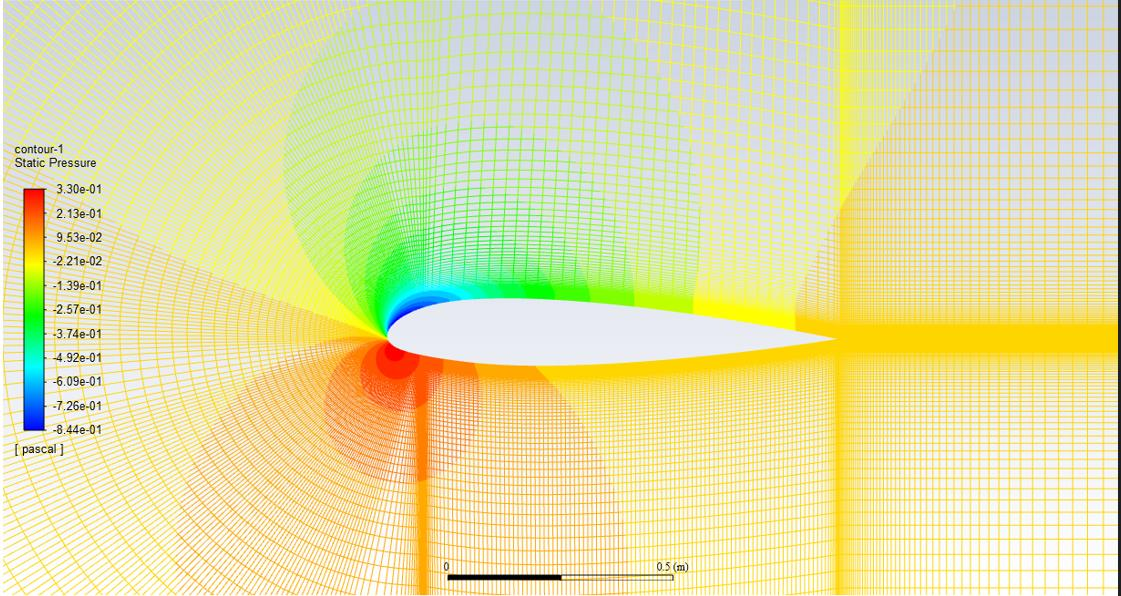
\includegraphics[width=\textwidth]{report_figures/static_pressure_aoa10.png}
        \caption{Static Pressure Contour at $\alpha = 10^\circ$}
    \end{subfigure}
    \caption{Static pressure field contours around the NACA 23015 airfoil at $\alpha = 6^\circ$ and $\alpha = 10^\circ$.}
    \label{fig:static_pressure}
\end{figure}

At $\alpha = 6^\circ$, the pressure distribution exhibits moderate suction along the upper surface with a gentle recovery gradient toward the trailing edge. At $\alpha = 10^\circ$, a localized, intense low-pressure core forms immediately behind the leading edge, while higher stagnation pressure develops along the lower pressure surface. This marked increase in net differential pressure ($\Delta p$) drives the higher lift coefficient. However, the steeper adverse pressure gradient on the aft upper surface at $\alpha = 10^\circ$ heralds incipient boundary layer deceleration.

\subsection{Dynamic Pressure Distribution}
Dynamic pressure ($q = \frac{1}{2}\rho |\vec{v}|^2$) distributions are compared in Figure~\ref{fig:dynamic_pressure}.

\begin{figure}[H]
    \centering
    \begin{subfigure}[b]{0.48\textwidth}
        \centering
        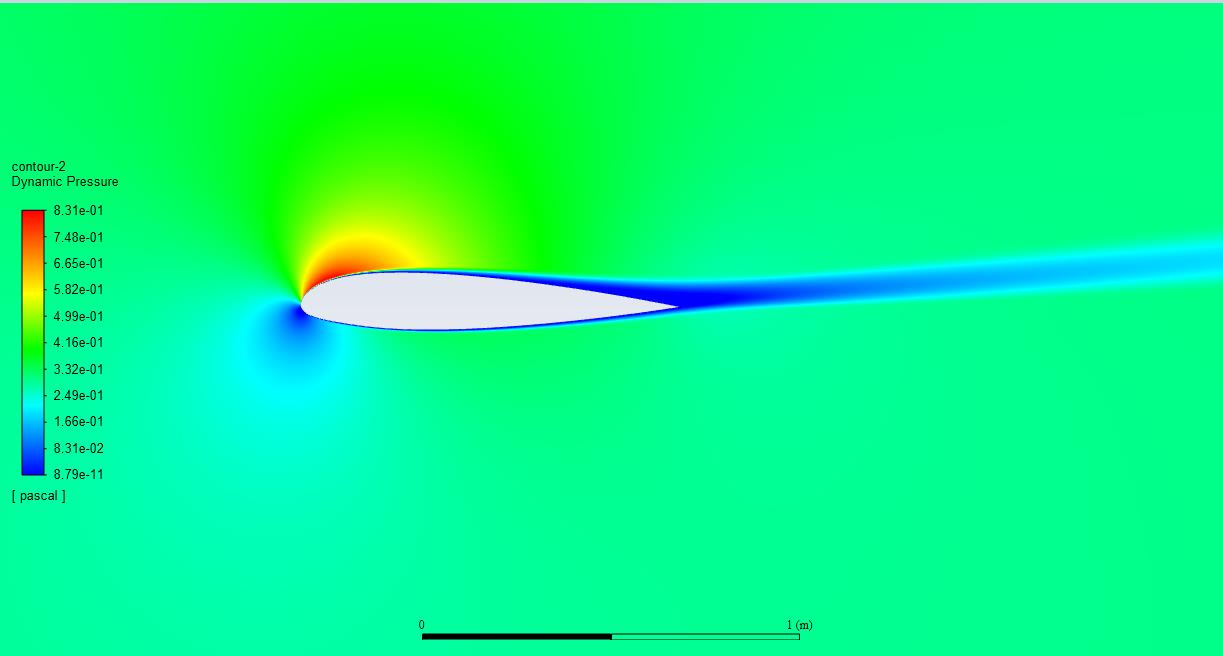
\includegraphics[width=\textwidth]{report_figures/dynamic_pressure_aoa6.png}
        \caption{Dynamic Pressure Contour at $\alpha = 6^\circ$}
    \end{subfigure}
    \hfill
    \begin{subfigure}[b]{0.48\textwidth}
        \centering
        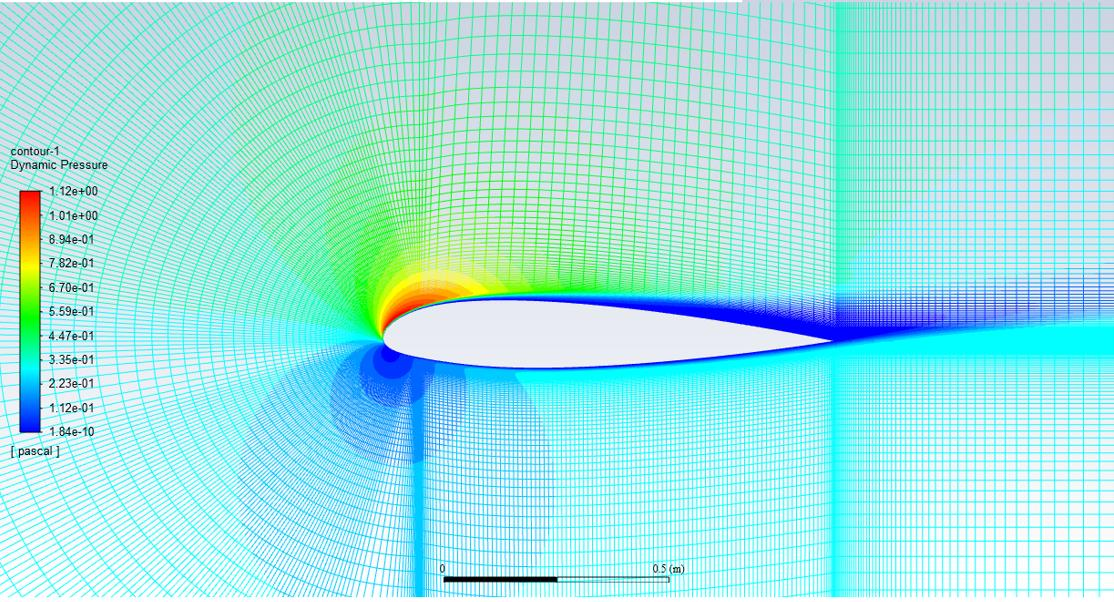
\includegraphics[width=\textwidth]{report_figures/dynamic_pressure_aoa10.png}
        \caption{Dynamic Pressure Contour at $\alpha = 10^\circ$}
    \end{subfigure}
    \caption{Dynamic pressure contours around the NACA 23015 airfoil at $\alpha = 6^\circ$ and $\alpha = 10^\circ$.}
    \label{fig:dynamic_pressure}
\end{figure}

At $\alpha = 6^\circ$, dynamic pressure remains uniformly distributed with moderate cresting over the upper surface. At $\alpha = 10^\circ$, an intense concentration of dynamic pressure manifests at the leading-edge suction crest due to high local flow acceleration, followed by a pronounced deficit along the aft upper surface where the boundary layer loses momentum.

\subsection{Velocity Magnitude Contours}
Velocity magnitude fields are presented in Figure~\ref{fig:velocity_contours}.

\begin{figure}[H]
    \centering
    \begin{subfigure}[b]{0.48\textwidth}
        \centering
        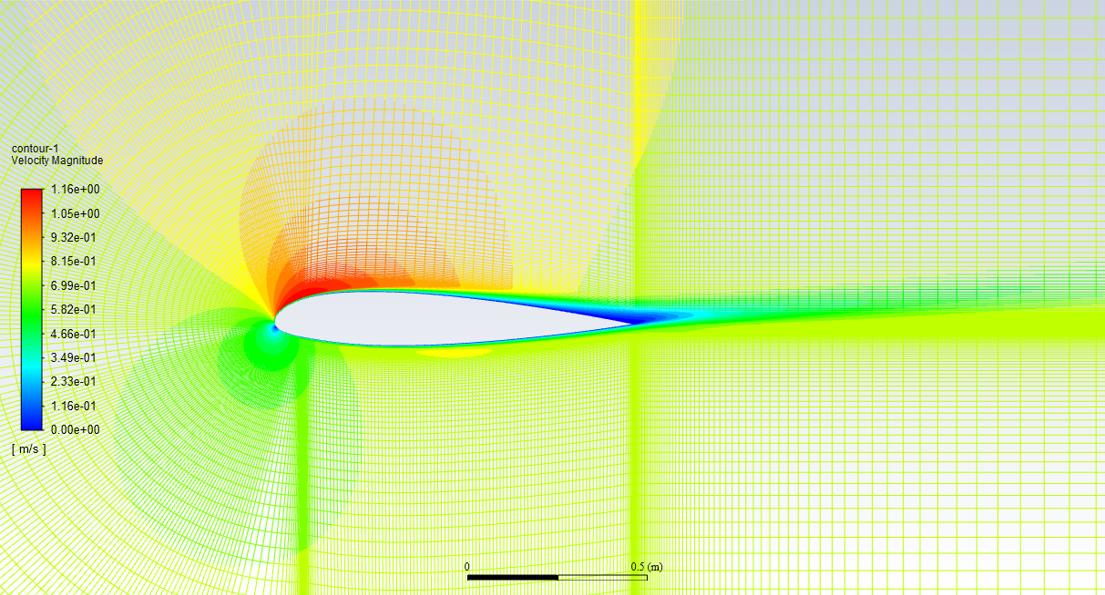
\includegraphics[width=\textwidth]{report_figures/velocity_aoa6.png}
        \caption{Velocity Magnitude at $\alpha = 6^\circ$}
    \end{subfigure}
    \hfill
    \begin{subfigure}[b]{0.48\textwidth}
        \centering
        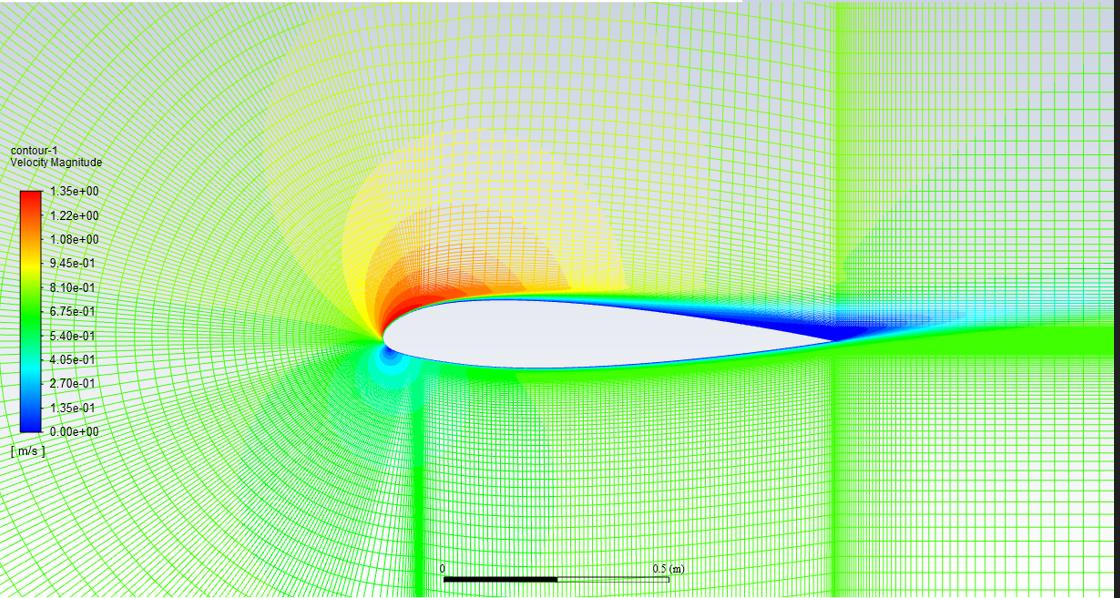
\includegraphics[width=\textwidth]{report_figures/velocity_aoa10.png}
        \caption{Velocity Magnitude at $\alpha = 10^\circ$}
    \end{subfigure}
    \caption{Velocity magnitude contours showing boundary layer development and wake formation.}
    \label{fig:velocity_contours}
\end{figure}

At $\alpha = 6^\circ$, the velocity field indicates smooth, attached flow across the entire chord with symmetric wake closure. At $\alpha = 10^\circ$, peak velocities exceed $1.35\text{ m/s}$ near the leading edge, and sharp velocity gradients emerge. Towards the trailing edge, a visible low-velocity deficit zone develops, confirming boundary layer thickening and expanded wake width.

\subsection{Vorticity Field and Shear Layer Dynamics}
Vorticity contours ($\vec{\omega} = \nabla \times \vec{v}$) in Figure~\ref{fig:vorticity_contours} delineate shear layer confinement.

\begin{figure}[H]
    \centering
    \begin{subfigure}[b]{0.48\textwidth}
        \centering
        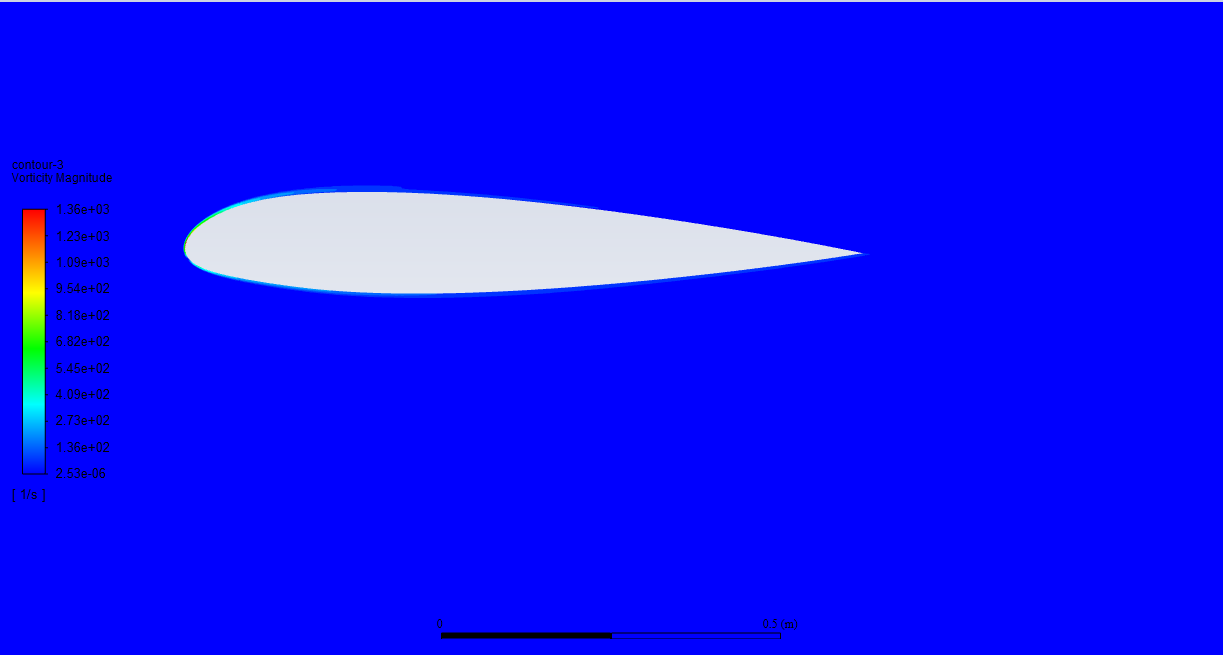
\includegraphics[width=\textwidth]{report_figures/vorticity_aoa6.png}
        \caption{Vorticity Contour at $\alpha = 6^\circ$}
    \end{subfigure}
    \hfill
    \begin{subfigure}[b]{0.48\textwidth}
        \centering
        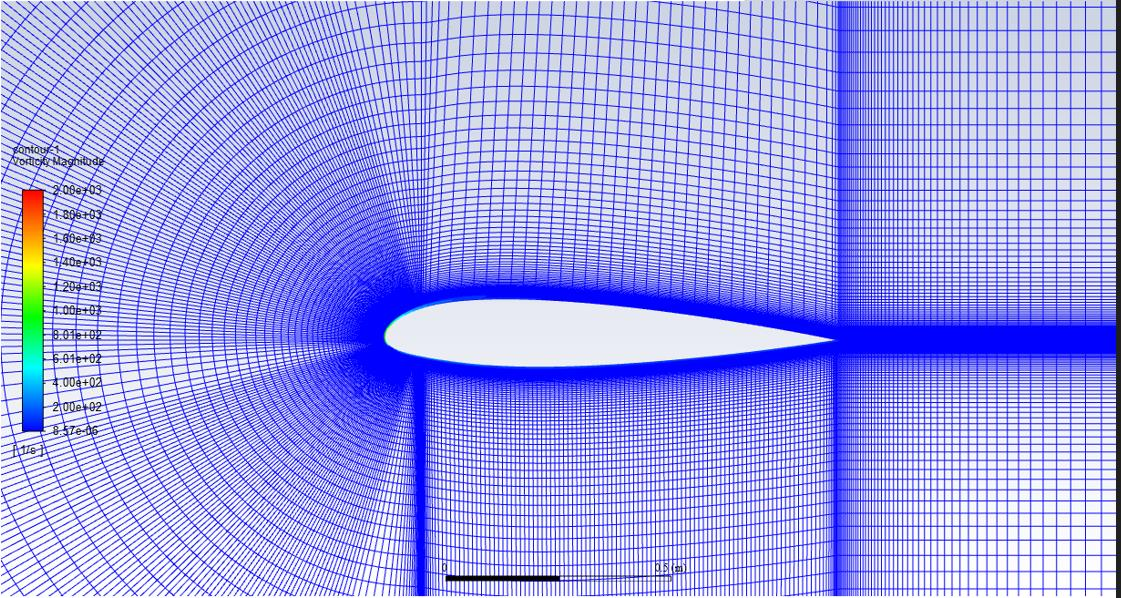
\includegraphics[width=\textwidth]{report_figures/vorticity_aoa10.png}
        \caption{Vorticity Contour at $\alpha = 10^\circ$}
    \end{subfigure}
    \caption{Vorticity contours showing boundary layer shear layer intensity and wake shedding.}
    \label{fig:vorticity_contours}
\end{figure}

At $\alpha = 6^\circ$, vorticity is tightly confined to an exceptionally thin near-wall layer with negligible vorticity shedding into the wake. At $\alpha = 10^\circ$, upper-surface vorticity production intensifies substantially, and viscous shear layers begin detaching into the wake, reflecting boundary layer destabilization.

\subsection{Streamline Patterns and Flow Topology}
Streamline patterns colored by the stream function are displayed in Figure~\ref{fig:streamlines}.

\begin{figure}[H]
    \centering
    \begin{subfigure}[b]{0.48\textwidth}
        \centering
        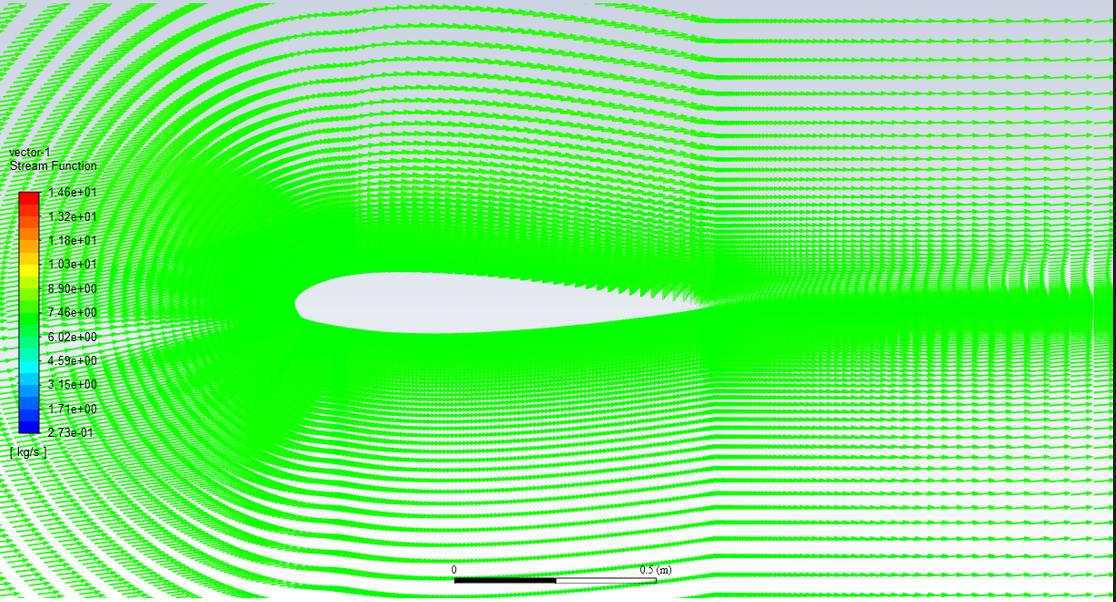
\includegraphics[width=\textwidth]{report_figures/streamlines_aoa6.png}
        \caption{Streamlines at $\alpha = 6^\circ$}
    \end{subfigure}
    \hfill
    \begin{subfigure}[b]{0.48\textwidth}
        \centering
        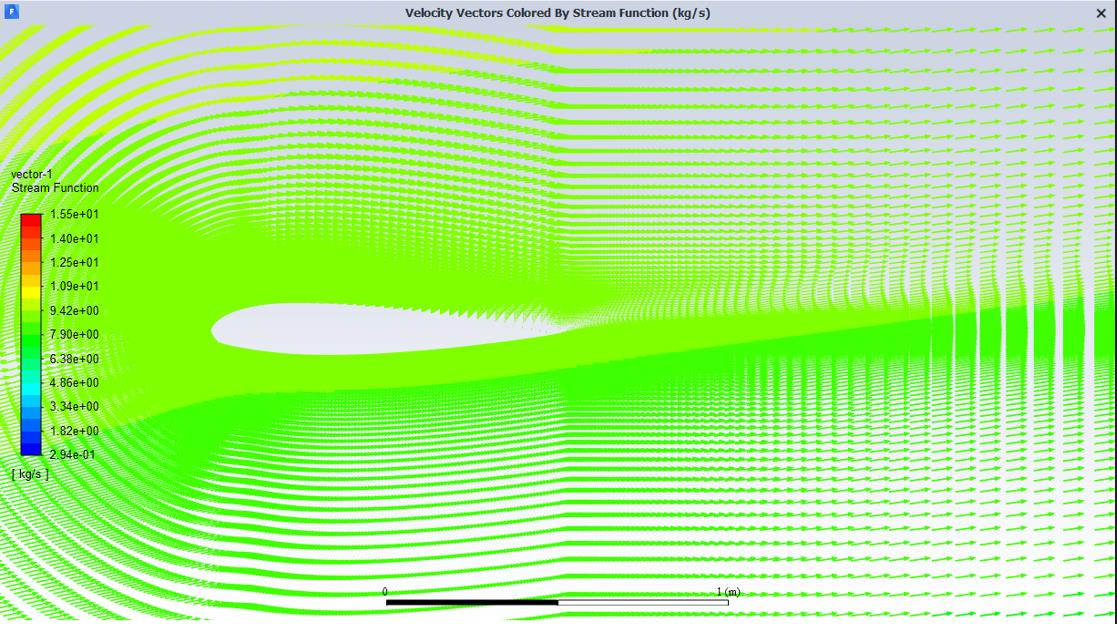
\includegraphics[width=\textwidth]{report_figures/streamlines_aoa10.png}
        \caption{Streamlines at $\alpha = 10^\circ$}
    \end{subfigure}
    \caption{Streamline trajectories colored by stream function illustrating flow conformity and aft divergence.}
    \label{fig:streamlines}
\end{figure}

At $\alpha = 6^\circ$, streamlines conform smoothly to the airfoil curvature along both surfaces. At $\alpha = 10^\circ$, the streamlines exhibit upward divergence and curvature deflection over the aft $25\%$ of the upper surface, signaling boundary layer displacement and the initial onset of recirculation.

\subsection{Surface Pressure Coefficient \texorpdfstring{($C_p$)}{(Cp)} Distributions}
The chordwise pressure coefficient distribution is defined as:
\begin{equation}
    C_p = \frac{p - p_\infty}{\frac{1}{2}\rho v_\infty^2}
\end{equation}
The resulting distributions along the upper and lower surfaces are shown in Figure~\ref{fig:cp_distributions}.

\begin{figure}[H]
    \centering
    \begin{subfigure}[b]{0.48\textwidth}
        \centering
        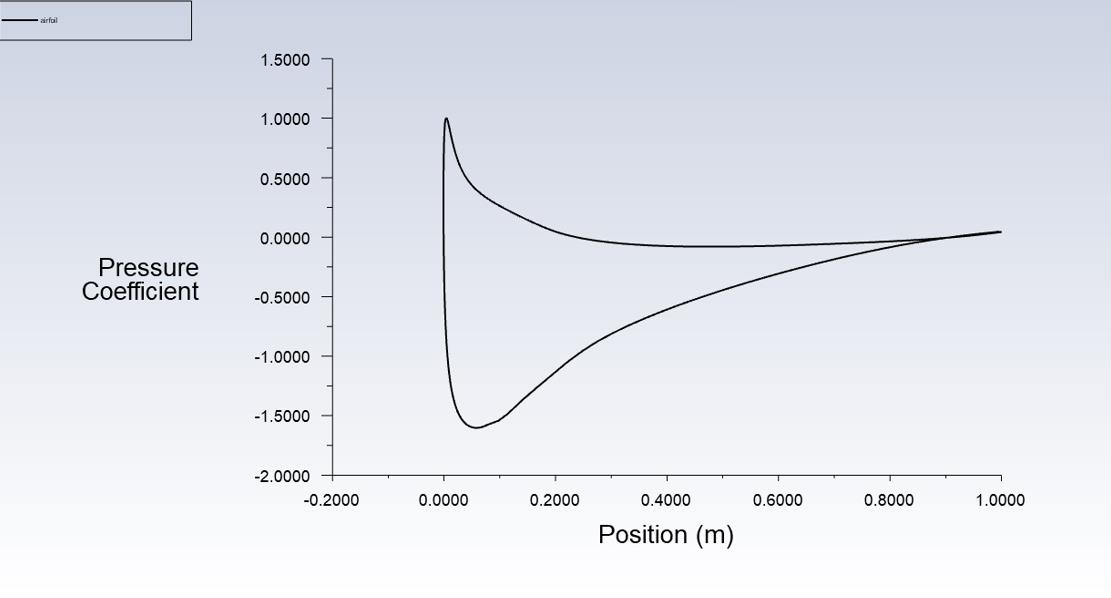
\includegraphics[width=\textwidth]{report_figures/cp_distribution_aoa6.png}
        \caption{$C_p$ vs. Chord Position ($x$) at $\alpha = 6^\circ$}
    \end{subfigure}
    \hfill
    \begin{subfigure}[b]{0.48\textwidth}
        \centering
        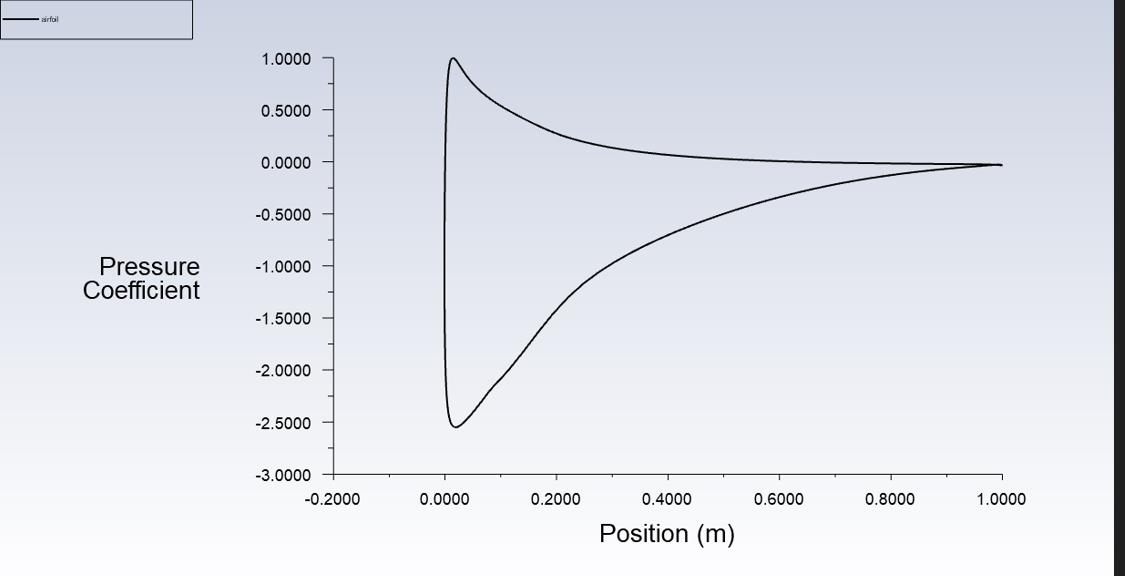
\includegraphics[width=\textwidth]{report_figures/cp_distribution_aoa10.png}
        \caption{$C_p$ vs. Chord Position ($x$) at $\alpha = 10^\circ$}
    \end{subfigure}
    \caption{Chordwise surface pressure coefficient ($C_p$) distributions at $\alpha = 6^\circ$ and $\alpha = 10^\circ$.}
    \label{fig:cp_distributions}
\end{figure}

At $\alpha = 6^\circ$, the enclosed area between the upper suction surface and lower pressure surface remains moderate, with a suction peak of $C_{p,\text{min}} \approx -1.6$. At $\alpha = 10^\circ$, the leading-edge suction peak drops sharply to $C_{p,\text{min}} \approx -2.55$, greatly increasing the enclosed loop area (directly proportional to section lift). The steeper adverse gradient ($dC_p/dx > 0$) towards the trailing edge at $\alpha = 10^\circ$ corresponds directly to boundary layer momentum loss.

% ==============================================================================
% SECTION 7: CONCLUSIONS
% ==============================================================================
\section{Conclusions}
In this numerical investigation, external flow over a 2D NACA 23015 airfoil was thoroughly simulated and analyzed using ANSYS Fluent 2019 R1. Key conclusions from the study include:
\begin{enumerate}
    \item \textbf{Grid Independence:} A mesh independence study verified that the medium mesh ($81,300$ elements) provides asymptotic grid convergence with an error of only $1.3\%$ relative to the fine grid ($199,500$ elements), while reducing computational runtime by over $50\%$.
    \item \textbf{Experimental Validation:} At $\alpha = 6^\circ$, the simulated lift coefficient ($C_l = 0.612$) agreed within $12.5\%$ of experimental wind tunnel benchmarks. Drag overprediction ($C_d = 0.028$ vs. $0.014$) was attributed to the absence of laminar-to-turbulent transition modeling in the standard $k\text{-}\omega\text{ SST}$ model.
    \item \textbf{Turbulence Physics:} Comparing laminar and turbulent models at $\alpha = 10^\circ$ verified the essential role of turbulent momentum transport in preventing premature boundary layer separation under strong adverse pressure gradients.
    \item \textbf{Angle of Attack Dynamics:} Elevating the angle of attack from $6^\circ$ to $10^\circ$ enhanced section lift by intensifying leading-edge suction ($C_{p,\text{min}}$ from $-1.6$ to $-2.55$), while also initiating aft boundary layer thickening, vorticity shedding, and wake expansion.
\end{enumerate}

\end{document}
